\subsection{Frozen Lake}
As presented in \cref{sec:intro}, Frozen Lake is the simplest scenario we considered for evaluating our solutions.

\subsubsection{NEAT}
Since the only information that can be sensed from the environment is the agent position, the final agent is overfitted on the map that is used in the training procedure. When working with the deterministic version of the environment (not slippery), this constraint allowed us to stop the evolution process once having at least one maximized topology with fitness equal to one.

We opted for a fully-connected NN in which each node is connected to every other node of the previous and next layer: one input value for the agent position and four outputs for the possible actions. The performed action is chosen by running the \texttt{argmax} function on the four output nodes. Once a single topology with fitness equal to one is found, the evolution process is stopped, since the optimal agent has been achieved.

Interestingly, the evolution process was not converging when dealing with a single input with range \([0,15]\) (using the 4x4 map) to describe the agent position. Therefore, we decided to encode it through one-hot encoding, in order to limit input values in the range \([0,1]\). In this case, after one or two generations with population size of 200, the optimal topology is found on the 4x4 grid size.

When enabling the slippery option, on our experiments it is impossible to find an optimal agent which is able to solve the environment consistently, since the intended action is not always performed.

\subsubsection{BT}
Also when using Behavior Trees, the agent is overfitted on the specific grid composition. Even though by looking at \cref{fig:fitness-bt-frozen-lake} it looks like that the maximum fitness value is never fully achieved, this happens because BTs can be penalized of a multiplicative factor (in this case \(0.01\)) on the number of nodes and tree depth. This prevents the exponential increase of the size that could occur as a result of recombination.

\begin{figure}
    \centering
    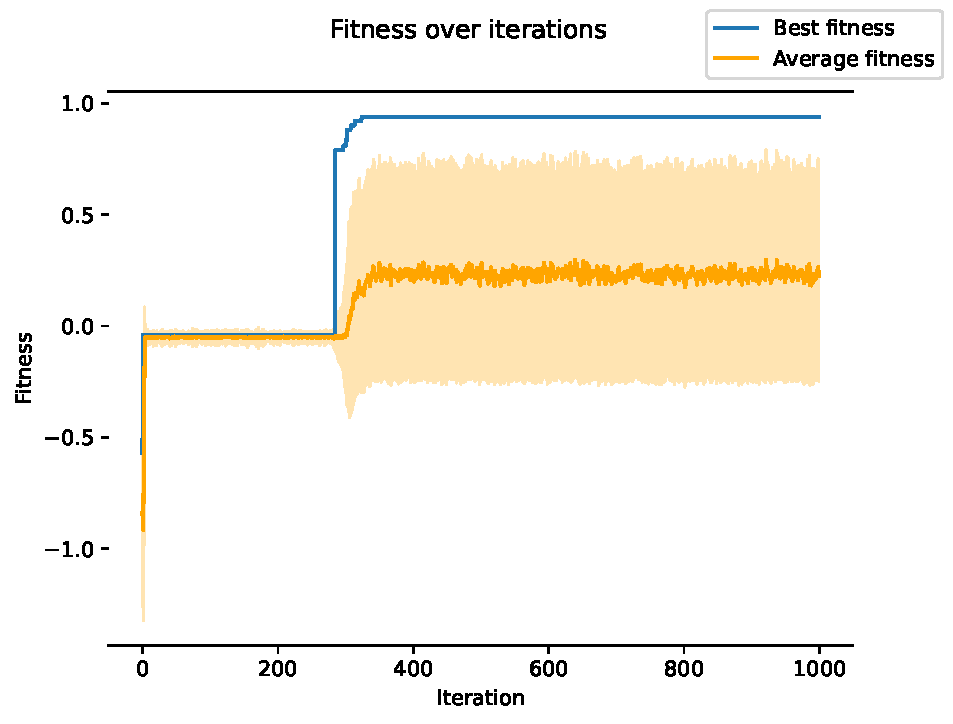
\includegraphics[width=0.8\linewidth]{./images/fitness_over_iterations_frozenlake_bt.pdf}
    \caption{Best and average fitness over iterations on Frozen Lake BT with std represented by the light orange area.}
    \label{fig:fitness-bt-frozen-lake}
\end{figure}

\subsection{Lunar Lander}
Lunar Lander is more complex with respect to Frozen Lake due to the increased number of variables involved. Results in this environment turned out to be not consistent since the fitness function receives a huge bump of 100 points when successfully landing in the pad.

\subsubsection{NEAT}
In this case, using the same Frozen Lake configuration NEAT is able to obtain good results as shown in \cref{fig:fitness-neat-lunar-lander}. Moreover, to make the final agent more stable, the score of an agent is computed by averaging the evaluation over five runs with different random seeds.

\begin{figure}
    \centering
    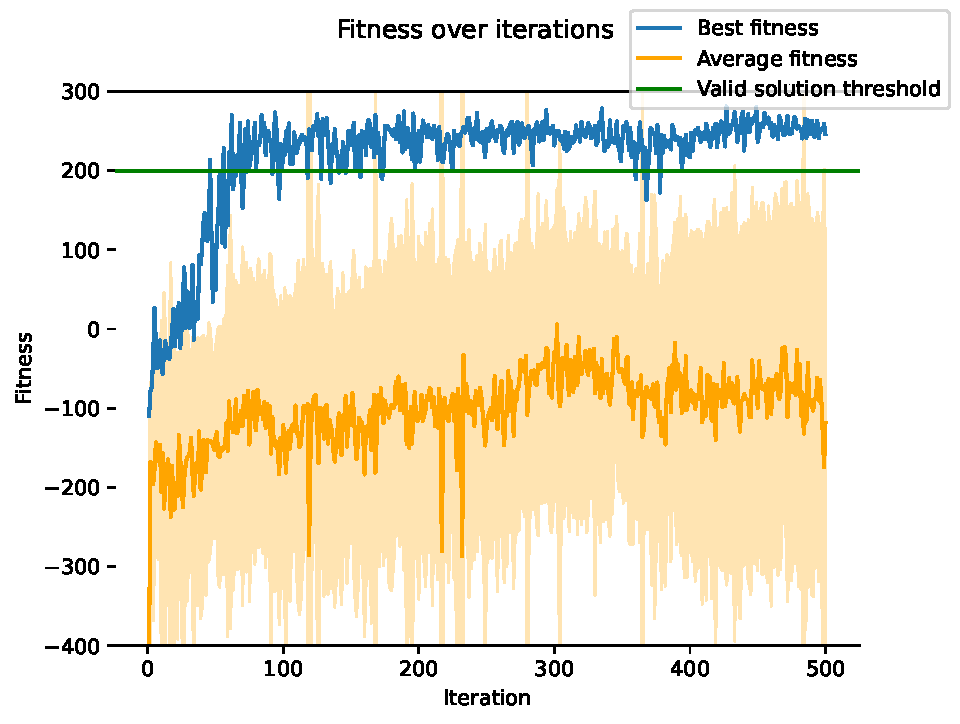
\includegraphics[width=0.8\linewidth]{./images/fitness_over_iterations_lunar_lander_neat.pdf}
    \caption{Best and average fitness over iterations on Lunar Lander NEAT with std represented by the light orange area.}
    \label{fig:fitness-neat-lunar-lander}
\end{figure}

\subsubsection{BT}
Similarly to NEAT, we started from the configuration used in Frozen Lake. In this case, in \cref{fig:fitness-bt-lunar-lander} we tested the environment with a single random seed, that influences the map creation and the initial inertia of the spaceship.

We noticed that the tree obtained was bloated with hundreds of nodes. In order to reduce the number of nodes and at the same time improve interpretability of the model, we added a metric that punishes the size of BTs. Additionally, we started tracking the percentage of active nodes: we then used this information to prune inactive nodes with \(0.05\) probability. Such a small percentage is chosen to guarantee some initial exploration of the search space through recombination of unused BT branches before starting the exploitation process.

\begin{figure}
    \centering
    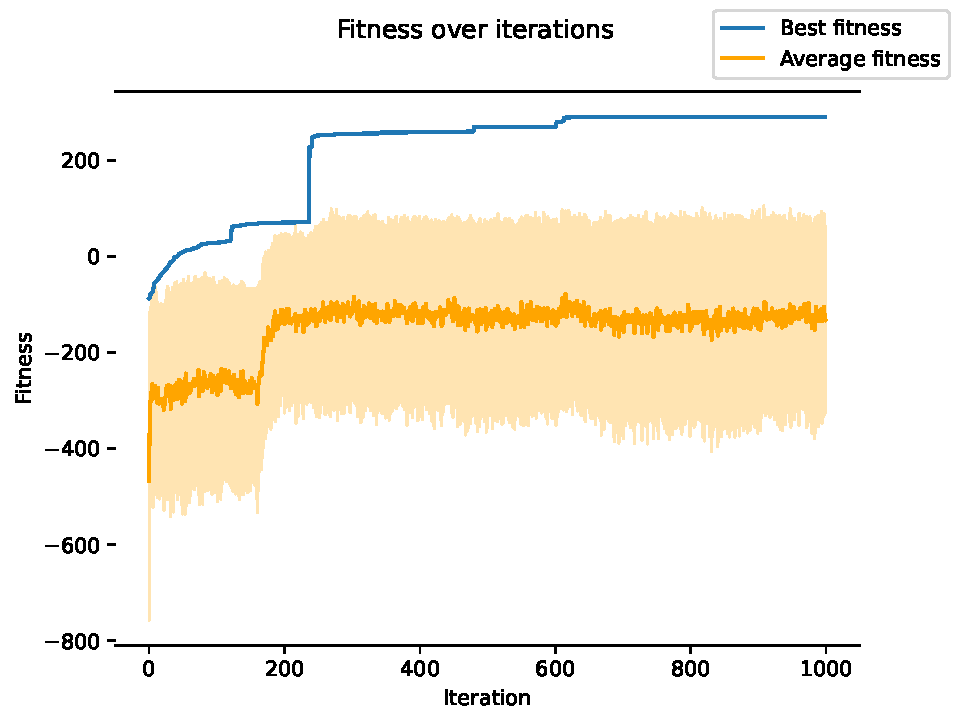
\includegraphics[width=0.8\linewidth]{./images/fitness_over_iterations_lunar_lander_bt.pdf}
    \caption{Best and average fitness over iterations on Lunar Lander BT with std represented by the light orange area.}
    \label{fig:fitness-bt-lunar-lander}
\end{figure}

However we noticed that the best BT is overfitted on the random seed used during the training phase and it is unable to land correctly with different initial conditions. We have tried to overcome this limitation by evaluating the fitness of a BT over different initial conditions (as we did in NEAT), but we found that this setup does not converge. This is could be a consequence of the fact that BT has a different evolution process with respect to NEAT since it does not cluster agents in species.

\subsection{Derk Gym}
Derk Gym is the most complex environment: we used it as a stretch goal to evaluate NEAT and our BT implementation.

\subsubsection{NEAT}
NEAT NNs receive as inputs from the environment 64 observation variables to produce 12 outputs, which grouped together enable the agent to move, rotate, chase, cast abilities, and focus targets: this configuration is called \texttt{64 input and 12 outputs}. Even though we performed extensive testings by tuning hyper parameters, the fitness scores showed an absence of an improving trend in the best fitness over subsequent generations, as can be seen in \cref{fig:fitness-neat-derk}. This could be related to the huge complexity of the search space and the consequential amount of time required for finding a potential optima.

% Therefore, as a second approach, we tried to reduce the input space only to the most important 13 variables. Additionally, we also modified the reward function to simplify the game dynamics. Unfortunately, the obtained results did not show an improvement and following this hypothesis we tried to shrink even more the problem size limiting the ability choice to only one item and removing the possibility of rotation and chase, this experiment was denominated \texttt{13 inputs and 10 outputs}.

Therefore, as a second approach, we tried to reduce the input space to the most important 13 variables and the output space by removing the possibility of rotation and chase. Additionally, we also modified the reward function to simplify the game dynamics and selected fixed abilities and weapons. We refer this experiment as \texttt{13 inputs and 10 outputs}. Unfortunately, also in this case the results were not promising.

\begin{figure}
    \centering
    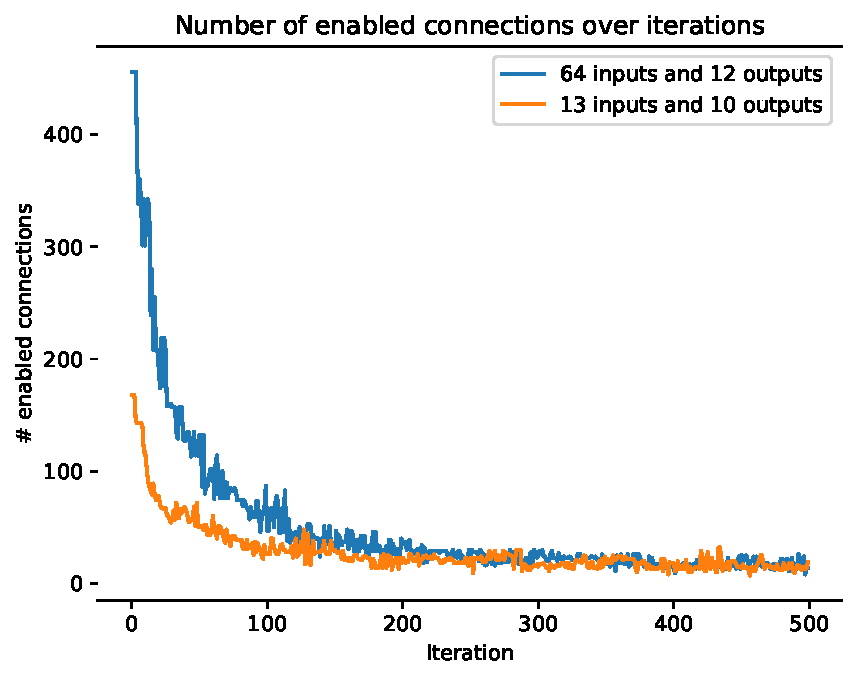
\includegraphics[width=0.8\linewidth]{./images/n_enabled_connections_over_iterations_derk_neat.pdf}
    \caption{Number of best network enabled connections over iteration Derk environment with NEAT solver.}
    \label{fig:enabled-connection-iteration-derk-neat}
\end{figure}

While investigating, we noticed that the number of enabled connections exponentially decreases over generations, as can be observed in \cref{fig:enabled-connection-iteration-derk-neat}. 
Since there is no correlation between the number of enabled connections and the number of nodes or the fitness value, we attributed the exponential decrease to the sparsity of the initial population. As already presented in \cref{sec:structural-complexity}, due to the dual optimization problem addressed during the NEAT evolution process, it would be better to start the evolution from simple structures. Therefore we simplified the initial topologies reducing the number of hidden layers and choosing different initial connection strategies, but the outcome was almost indistinguishable.

By looking at Reinforcement Learning state-of-the-art solutions, we then moved to a different approach based on Q-learning~\cite{DEEPQL}, in which each output node represents a single possible action that can be taken by an agent. In this case, the action space is composed of almost $1000$ possible actions obtained by linearly sampling the output space: a topology that requires so many output nodes should also have a deep structure. The increased size of topologies brought to the already known explosion of complexity: even with this attempt there was no visible improving trend over generations in terms of best fitness.

Alternatively, we attempted to reduce the action space to a limited set of 25 pre-computed actions, with the goal of simplify as much as possible the Q-learning problem. This last approach did not work as well, as presented in \cref{fig:fitness-neat-derk}.

% TODO: perche' il 25 action non funziona come dovuto e ha best fitness sempre vicina a zero?

\subsubsection{BT}
Also with BTs, we tested different evolutionary algorithms varying different hyper parameters and reducing the evolution space, but we quickly realized that all approaches were failing similarly to NEAT, as shown in \cref{fig:fitness-bt-derk}.

\begin{figure}
    \centering
    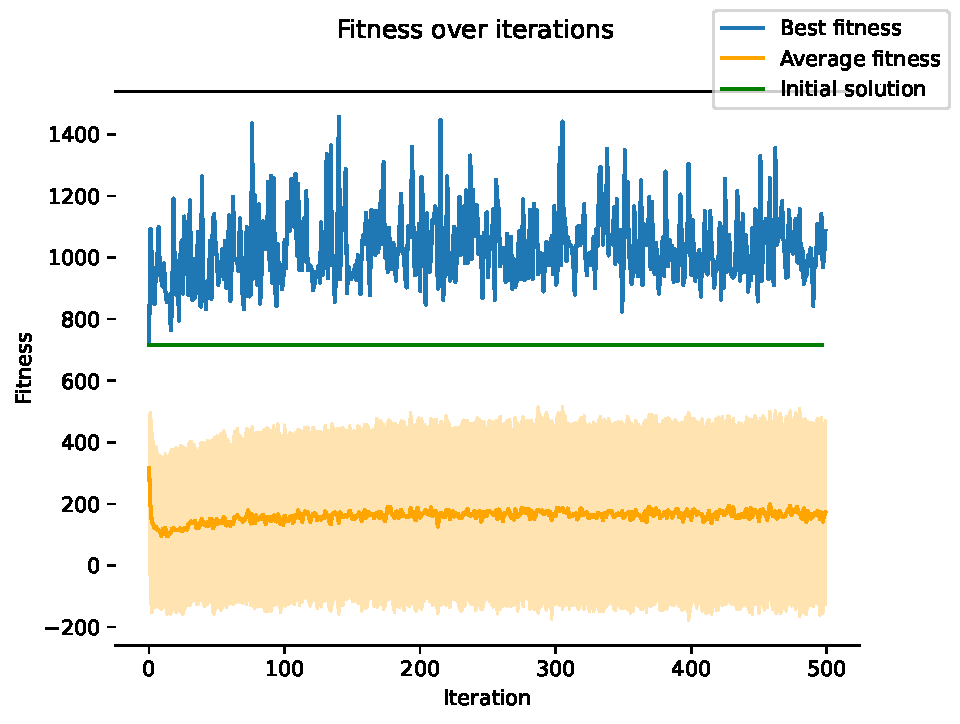
\includegraphics[width=0.8\linewidth]{./images/fitness_over_iterations_derk_bt.pdf}
    \caption{Best and average fitness over iterations on Derk BT with std represented by the light orange area.}
    \label{fig:fitness-bt-derk}
\end{figure}

Since BTs are intepretable, we have tried handcrafting simple BTs testing different tree topologies. This helped us in debugging the environment and discover that some actions may return no feedback: for example the gun does not shoot if the target is not in a certain range. This lack of feedback is a crucial missing step on modelling complex behaviors with BTs, since action nodes should be able to return whether the action succeeded or not.

In addition to this, we also discovered that some actions may take many environment steps to be fully performed: for example a bullet takes time to reach the enemy which depends on the distance.
This implies that the instantaneous agent reward is not always related to action just performed, but also to some past actions.

Moreover, we handcrafted a BT that chases enemies and their tower if not in range, shoots at them until their HP is down to 0. Then we tried to initialize the BT evolution process with this tree, but after some generations the outcomes were similar to the ones with random initialization.
